%%% Exemplo de utilização da classe ITA
%%%
%%%   por        Fábio Fagundes Silveira   -  ffs [at] ita [dot] br
%%%              Benedito C. O. Maciel     -  bcmaciel [at] ita [dot] br
%%%              Giovani Volnei Meinertz   -  giovani [at] ita [dot] br
%%%    	         Hudson Alberto Bode       -  bode [at] ita [dot]br
%%%    	         P. I. Braga de Queiroz    -  pi [at] ita [dot] br
%%%    	         Jorge A. B. Gripp         -  gripp [at] ita [dot] br
%%%    	         Juliano Monte-Mor         -  jamontemor [at] yahoo [dot] com [dot] br
%%%    	         Tarcisio A. B. Gripp      -  tarcisio.gripp [at] gmail [dot] com
%%%    	         
%%%
%%%  IMPORTANTE: O texto contido neste exemplo nao significa absolutamente nada.  :-)
%%%              O intuito aqui eh demonstrar os comandos criados na classe e suas
%%%              respectivas utilizacoes.
%%%
%%%  Tese.tex  2015-04-08
%%%  $HeadURL: http://www.apgita.org.br/apgita/teses-e-latex.php $
%%%
%%% ITALUS
%%% Instituto Tecnológico de Aeronáutica --- ITA, Sao Jose dos Campos, Brasil
%%%                   http://groups.yahoo.com/group/italus/
%%% Discussion list: italus {at} yahoogroups.com
%%%
%++++++++++++++++++++++++++++++++++++++++++++++++++++++++++++++++++++++++++++++
% Parametros da classe ITA para inserir em \documentclass[?]{?}
%   tg       = Trabalho de Graduacao
%   tgfem    = Para Engenheiras
%   msc      = Dissertacao de Mestrado
%   mscfem   = Para Mestras
%   dsc      = Tese de Doutorado
%   dscfem   = Para Doutoras
%   quali    = Exame de Qualificacao
%   qualifem = Exame de Qualificacao para Doutoras
%   dv       = 'Draft Version'     --> imprime 'Versao Preliminar + data no rodape
%   eng      = para teses em inglês
%++++++++++++++++++++++++++++++++++++++++++++++++++++++++++++++++++++++++++++++
%se fosse em inglês: \documentclass[dsc, eng]{ita}
%para ``draft version'': \documentclass[dsc, dv]{ita} ou \documentclass[dsc, eng, dv]{ita}

\documentclass[tg]{ita}    % ITA.cls based on standard book.cls 
% Quando alterar a classe, por exemplo de [msc] para [msc, eng]) rode mais uma vez o botão BUILD OUTPUT caso haja erro
\usepackage{ae}
\usepackage{graphicx}
\usepackage{epsfig}
\usepackage{amsmath}
\usepackage{amssymb} 
\usepackage{subfig}
\usepackage{multirow}
\usepackage{float}

%++++++++++++++++++++++++++++++++++++++++++++++++++++++++++++++++++++++++++++++
% Espaçamento padrão de todo o documento
%++++++++++++++++++++++++++++++++++++++++++++++++++++++++++++++++++++++++++++++
\onehalfspacing

%singlespacing Para um espaçamento simples
%onehalfspacing Para um espaçamento de 1,5
%doublespacing Para um espaçamento duplo

%++++++++++++++++++++++++++++++++++++++++++++++++++++++++++++++++++++++++++++++
% Identificacoes (se o trabalho for em inglês, insira os dados em inglês)
% Para entradas abreviadas de Professora (Profa.) em português escreva: Prof$^\textnormal{a}$.
%++++++++++++++++++++++++++++++++++++++++++++++++++++++++++++++++++++++++++++++
\course{Engenharia de Computação} % Programa de PG ou Curso de Graduação
\dept{Engenharia de Computação} % Divisão Acadêmica no ITA

% Autor do trabalho: Nome Sobrenome
\authorgender{masc}                     %sexo: masc ou fem
\author{Gustavo Ceci}{Guimarães}
\itaauthoraddress{Rua H8B 238}{12.228-461}{São José dos Campos--SP}

% Titulo da Tese/Dissertação
\title{Desenvolvimento de uma framework em C++ para criação de jogos 3d para a Web}

% Orientador
\advisorgender{masc}                    % masc ou fem
\advisor{Prof.~Dr.}{Edgar Toshihiro Yano}{ITA}

%Coordenador do curso no caso de TG
\bosscoursegender{fem}									% masc ou fem
\bosscourse{Prof.~Dr.}{Cecilia César}

% Palavras-Chaves informadas pela Biblioteca -> utilizada na CIP
\kwcip{Jogos}
\kwcip{WebGL}
\kwcip{OpenGL}
\kwcip{WebAssembly}
\kwcip{Emscripten}
\kwcip{C++}

% membros da banca examinadora

% Data da defesa (mês em maiúsculo, se trabalho em inglês, e minúsculo se trabalho em português) 
\date{22}{novembro}{2017}

% TODO: Número CDU - (somente para TG)
\cdu{621.38}

% Glossario
\makeglossary
\frontmatter

\begin{document}
% Folha de Rosto e Capa para o caso do TG
\maketitle

% Dedicatoria: Nao esqueca essa secao  ... :-)
\begin{itadedication}
Aos meus queridos amigos
\end{itadedication}

% Agradecimentos
\begin{itathanks}
Primeiramente, gostaria de agradecer ao Dr. Donald E. Knuth, por ter desenvolvido o \TeX.

Ao Dr. Leslie Lamport, por ter criado o \LaTeX, facilitando muito a utilização do \TeX, e assim, eu não ter que usar o Word.

Ao Prof. Dr. Meu Orientador, pela orientação e confiança depositada na realização deste trabalho.

Ao Dr. Nelson D'Ávilla, por emprestar seu nome a essa importante via de trânsito na cidade de São José dos Campos.

Ah, já estava esquecendo... agradeço também, mais uma vez ao \TeX, por ele não possuir vírus de macro :-)

\end{itathanks}

% Epígrafe
\thispagestyle{empty}
\ifhyperref\pdfbookmark[0]{\nameepigraphe}{epigrafe}\fi
\begin{flushright}
\begin{spacing}{1}
\mbox{}\vfill
{\sffamily\itshape
Não tem como dar errado.
}
\end{spacing}
\end{flushright}

% Resumo
\begin{abstract}
Aqui começa o resumo do referido trabalho. Não tenho a menor idéia do que colocar aqui. Sendo assim, vou inventar. Lá vai: Este trabalho apresenta uma metodologia de controle de posição das juntas passivas de um manipulador subatuado de uma maneira subótima. O termo subatuado se refere ao fato de que nem todas as juntas ou graus de liberdade do sistema são equipados com atuadores, o que ocorre na prática devido a falhas ou como resultado de projeto. As juntas passivas de manipuladores desse tipo são indiretamente controladas pelo movimento das juntas ativas usando as características de acoplamento da dinâmica de manipuladores. A utilização de redundância de atuação das juntas ativas permite a minimização de alguns critérios, como consumo de energia, por exemplo.
Apesar da estrutura cinemática de manipuladores subatuados ser idêntica a do totalmente atuado, em geral suas caraterísticas dinâmicas diferem devido a presença de juntas passivas. Assim, apresentamos a modelagem dinâmica de um manipulador subatuado e o conceito de índice de acoplamento. Este índice é utilizado na sequência de controle ótimo do \mbox{manipulador}.
A hipótese de que o número de juntas ativas seja maior que o número de
passivas  $(n_{a} > n_{p})$  permite o controle ótimo das juntas passivas, uma vez que na etapa
de controle destas há mais entradas (torques nos atuadores das juntas ativas), que
elementos a controlar (posição das juntas passivas). 
\end{abstract}

% Abstract
\begin{englishabstract}

Well, the book is on the table. This work presents a control methodologie for the position of the  passive joints of an underactuated manipulator in a suboptimal way. The term underactuated refers to the fact that not all the joints or degrees of freedom of the system are equipped with actuators, which occurs in practice due to failures or as design result. The passive joints of manipulators like this are indirectly controlled by the motion of the active joints using the dynamic coupling characteristics. The utilization of actuation redundancy of the active joints allows the minimization of some criteria, like energy consumption, for example. Although the kinematic structure of an underactuated manipulator is identical to that of a similar fully actuated one, in general their dynamic characteristics are different due to the presence of passive joints. Thus, we present the dynamic modelling of an underactuated manipulator and the concept of coulpling index. This index is used in the sequence of the optimal control of the manipulator.

\end{englishabstract}

% Lista de figuras
\listoffigures %opcional

% Sumario
\tableofcontents

\mainmatter
% Os capitulos comecam aqui

\chapter{Introdução}

A indústria de jogos é um dos setores da indústria de entretenimento que mais gera lucro, gerando em 2016 mais lucro que o setor de musica e de filmes \cite{NASDAQ}. Essa indústria é dividida em diversos outros subsetores como o desenvolvimento de jogos para video-game, jogos mobile e jogos de computador. Dentro do setor dos jogos de computador pode-se tambem fazer algumas subdivisões como jogos que precisam ser instalados e jogos que podem ser jogados no browser.

Apesar de ser a menor parcela do setor no quesito de lucro, os jogos de browser ainda possuem relevância no contexto geral, e muitas vezes servem como o ambiente inicial onde o jogo pode ser jogado \cite{NEWZOO}. Por não necessitarem de software baixado além do navegador e serem tipicamente gratuitos, os jogos de browser são de acessibilidade muito simples para o usuário. Para os desenvolvedores, especialmente aqueles sem investimentos multimilionários voltados para marketing e publicação, a acessibilidade dos jogos de browser torna-se um método de veículação e engajamento de usuário muito eficiente. Diversos jogos independentes bem sucedidos possuem ou possuiram em algum momento alguma versão ou protótipo possivel de ser jogado no browser \cite{BOI, CLICKERHEROES, SUPERHOT}.

Além do apelo financeiro, jogos podem ser usados como forma de expressão artística e como um hobby. Como para as grandes empresas jogos são um investimento multimilionário, os resultados são em sua maioria jogos menos inovadores que aqueles desenvolvidos por pequenas empresas ou desenvolvedores que o fazem por hobby, uma vez que o risco envolvido para estes costuma ser bem menor \cite{CREATINGGAMES}.

Inicialmente, grande parte dos jogos de browser eram desenvolvidos utilizando-se a ferramenta Adobe Flash, porém, com o surgimento do HTML5 e do WebGL, o uso de um plugin terceirizado para rodar jogos tem sido cada vez mais mal visto, incentivando o desenvolvimento usando as tecnologias padrão encontradas no browser \cite{UNITYWEB, FLASH}.

Uma limitação sempre presente quanto à evolução dos jogos de browser é a limitação da velocidade de processamento do browser, especialmente quando os jogos são em ambientes tridimensionais. A linguagem mais utilizada para o desenvolvimento de jogos 3d é C++, especialmente devido à eficiência, gerenciamento de memória e comunicação com sistemas de baixo nível como a placa de video. Como javascript é a linguagem padrão dos browsers e sua eficiência é consideravelmente inferior à de C++ \cite{BENCHMARK}, a implementação de jogos 3d com graficos otimizados no browser sempre foi deixada de lado. No entanto com o crescimento cada vez maior das tecnologias dos browsers tornou-se necessário cada vez mais ter códigos mais eficientes e com velocidades mais próximas à nativa, surgindo assim diversas soluções para se executar codigos nativos no browser como PNaCL \cite{PNACL} e WebAssembly \cite{WASM}.

\section{Motivação}

As ferramentas existentes hoje em dia para desenvolvimento de jogos com suporte para exportar para web são em sua maioria Engines completas, como Unity3d, Unreal Engine e Godot. Estas possuem inúmeras utilidades como simulação de física, criação de interface de usuário (UI), gerenciador de animações para modelos 3d, entre outras. Para ser possível a união de tantas ferramentas em uma unica Engine, o usuário acaba se vinculando demais à arquitetura da mesma e soluções improváveis acabam se tornando mais difíceis de se implementar devido à generalização. Para a maioria dos casos a Engine serve perfeitamente ao desenvolvedor, no entanto, em alguns casos a falta de controle é relevante.

Esse trabalho tem como objetivo criar não uma engine, mas uma framework que dá ao usuário a capacidade de pular as tarefas mais complicadas de se desenvolver uma engine, como um mecanismo simples de input e uma interface mais simples de utilização da placa de vídeo que o OpenGL padrão.

A motivação pessoal para o desenvolvimento desse trabalho é poder ter uma ferramenta propria para desenvolvimento de jogos, com capacidade de exportar para Web. Além disso, esse projeto visa ampliar os conhecimentos sobre os sistemas de baixo nível no desenvolvimento de jogos, especialmente um melhor entendimento de API's de gráfico 3d e da linguagem C++ em um projeto de maior escala.

\section{Objetivo}

O objetivo do trabalho é ter uma framework de facil distribuição e fácil uso no sistema operacional Windows. Para a criação de jogos, a framework terá como objetivo abstrair as camadas de entendimento complexo relacionado ao uso do OpenGL e do STL. A framework deverá ter uma interface simples de posicionamento de formas geométricas no espaço (sendo um bonus a possibilidade de se importar modelos 3d) além da implementação de um sistema de cameras básico. Além disso, a framework deverá possuir uma interface simples de leitura de input do teclado e do mouse. Por fim, caso se mostre necessário, a framework poderá ter integrada uma biblioteca de UI imediata para casos de debug e desenvolvimento.

\section{Ferramentas}
%Sequencia de passos necessários para demonstrar que o objetivo proposto foi atingido, ou seja, que os resultados obtidos são convincentes
\subsection{Emscripten}
Emscripten é um compilador de LLVM para javascript. LLVM é uma infraestrutura de compilador que serve para facilitar a criação de compiladores e transpiladores. Dada qualquer linguagem compilada para a linguagem intermediária do LLVM, a ferramenta Emscripten pode ser utilizada para ser enfim compilada pra javascript \cite{EMSCRIPTEN}.

O principal objetivo de compilar LLVM para javascript é a compilação de C++. Além disso, o Emscripten possui já implementadas algumas bibliotecas importantes para o uso no browser, sendo elas a transformação de OpenGL para WebGL e a biblioteca SDL2.

\subsection{OpenGL}
OpenGL, \textit{Open Graphics Library} é uma API multiplataforma padrão para desenvolvimento de graficos 3D. É um padrão de API 3D amplamente aceito com uso significante no mundo real.\cite{OPENGL}. A versão do OpenGL usada nos browsers, com a API em javascript é conhecida como WebGL, que é baseada no OpenGL ES 2.0, versão essa voltada para dispositivos móveis e sistemas embarcados. Como o emscripten é capaz de transformar um subconjunto de OpenGL ES 2.0 em WebGL sem maiores problemas \cite{EMSCRIPTEN_OPENGL}, esse será o subconjunto utilizado no projeto.

\subsection{SDL2}
SDL2, \textit{Simple DirectMedia Layer} é uma biblioteca de desenvolvimento multiplataforma criada para prover acesso de baixo nível aos hardwares de audio, mouse, teclado, joystick, alem de possuir uma interface com OpenGL \cite{SDL2}. Como é uma biblioteca muito utilizada para desenvolvimento de jogos em C++ e o emscripten já possui uma versão própria da biblioteca já compilada, essa foi a escolha de biblioteca base para a multimídia do trabalho.
\chapter{Desenvolvimento}
\label{cap:desenvolvimento}

\section{Hello World}

A primeira funcionalidade que foi implementada no projeto foi utilizar-se da biblioteca OpenGL e seguir os passos iniciais para ser possivel desenhar um triangulo na tela. 

Para isso foi implementada uma funcionalidade basica de criação de janela, utilizando-se do SDL2 para que isso fosse multiplataforma e funcionasse com o compilador do Emscripten.

Em seguida foram criadas classes básicas para a criação de shaders, código necessário para que os vertices e pixels da tela sejam coloridos. Após a capacidade de criação de shaders, os pontos de um triangulo foram colocados no loop principal do programa, e utilizando das funções do OpenGL, foi possível renderizar um triangulo conforme a figura \ref{des:glhello}.

\begin{figure}[]
  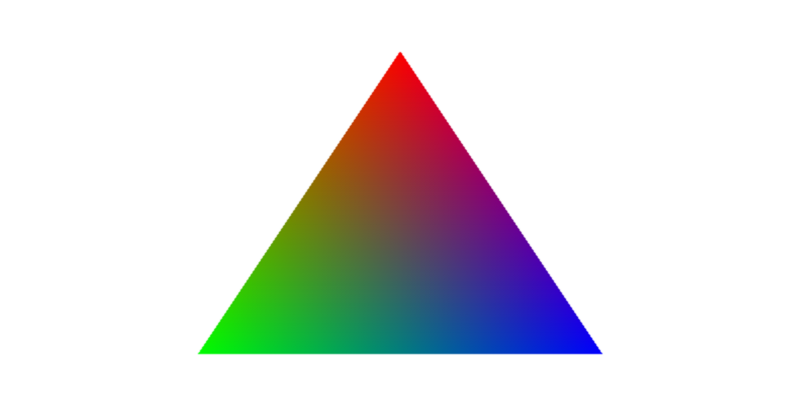
\includegraphics[width=\linewidth]{Cap-Desenvolvimento/glhello.png}
  \caption{Hello World do OpenGL}
  \label{des:glhello}
\end{figure}

\section{Criação de modelos}

A partir do momento que era possivel renderizar um triangulo, a renderização de uma lista de triangulos tornou-se trivial. Assim, o proximo passo do desenvolvimento foi fazer uma função que renderizasse uma lista de vértices quaisquer de um modelo para que fosse possivel renderizar vários ao mesmo tempo.

Para teste da criação de multiplos modelos, foi escrita à mão um array que continha todos os vertices dos triangulos de um cubo, e assim surgiu a primeira versão da função de desenhar cubos.

Em seguida para que multiplos objetos pudessem utilizar do mesmo modelo, mas serem posicionados em lugares diferentes da tela, foi implementada uma matriz de modelo, utilizando-se dos conceitos explicados no apendice \nameref{ape:matrix}

A cada vértice de um modelo é aplicada a transformação definida pela seguinte matriz:

\begin{equation}
  M = T * R * S
\end{equation}

Onde $T$ é a translação do modelo, $R$ é a rotação do modelo e $S$ é a escala do modelo. Assim, para cada modelo novo é enviada a matriz dele para o shader de vértices e nesse shader cada vértice é multiplicado por essa matriz.


\section{Criação de uma camera com perspectiva}

Após a possibilidade de criação e posicionamento de modelos, a proxima coisa importante de ser implementada seria uma camera, para primeiramente poder renderizar a cena vista de diversas posições e também para poder utilizar da perspectiva e os jogos criados parecerem verdadeiramente tridimensionais.

Primeiramente a ideia de mostrar a cena sendo vista de uma posição diferente a ideia principal é mover o mundo em relação à camera. Dessa forma, dado que a camera tenha uma translação $T_c$ e uma rotação $R_c$, podemos definir uma matriz que muda os objetos da sua posição no espaço para sua posição em relação à camera como:

\begin{equation}
  V = (T_c * R_c)^{-1}
\end{equation}

A matriz $V$ é conhecida como matriz \textit{View}. Para todos os objetos agora, multiplica-se todos os vértices do seu modelo pela matriz do modelo, e em seguida pela matriz $V$, fazendo com que todos se posicionem em relacao à camera.

O proximo passo foi implementar a camera visualizar a cena com uma perspectiva tridimensional, para isso utilizando-se dos conceitos explicados no apendice \nameref{ape:matrix}, da matriz de perspectiva, tem-se a matriz $P$ e portanto, surge agora uma matriz muito importante, que transforma um modelo em um objeto em perspectiva no espaço em relação à camera.

\begin{equation}
  MVP = P * V * M
\end{equation}

Essa matriz é constantemente atualizada, toda vez que a camera se move, e enviada para a GPU para cada objeto a ser renderizado. Com ela toda a renderização 3d se torna possível e para criar as classes relacionadas à renderização 3d (Graphics, Camera, Transform) bastou-se separar as diferentes funcionalidades que deveriam ser publicas e separar as tarefas para cada parte diferente do projeto.

Em seguida, para testar alguns conceitos, a biblioteca gráfica foi expandida para mais próxima de sua versão final, com uma implementação simples de iluminação difusa e especular.

\section{Input do Usuário}

Após a implementação da biblioteca grafica, o proximo passo para tornar a imagem renderizada em um jogo seria a capacidade do código levar os inputs do usuário em consideração. Para a entrega inicial, foi implementado apenas input do mouse e do teclado.

A primeira coisa a ser implementada para o sistema de input era um sistema ainda mais genérico e que é util em diversos contextos de um jogo, um sistema de eventos. Nesse sistema podem ser atribuidas funções relacionadas a um evento e quando esse evento é disparado, todas as funções são chamadas.

Dado um sistema de eventos funcional, utilizando-se de ferramentas proporcionadas pela biblioteca SDL2, a implementação do sistema de input do usuario por eventos foi simples.

Por fim, para ser possíver fazer ações com consequencias depois de um determinado intervalo de tempo, foi implementada uma classe simples de callbacks temporais, na qual é possível dizer um tempo e uma função, e esta será chamada depois do tempo.

\section{Provas de Conceito}

Paralelo ao desenvolvimento da framework, alguns demos de uso da mesma foram sendo desenvolvidos. O mais elaborado deles foi um jogo em primeira pessoa no qual existem alguns cubos se movendo no espaço, um paralelepipedo sempre no centro da camera. Nesse jogo WASD é utilizado para se movimentar, o mouse serve para rodar a camera em relação ao eixo y e o clique do mouse atira pequenos cubos vermelhos. A figura \ref{des:gamedoom} mostra uma imagem do jogo.

\begin{figure}[]
  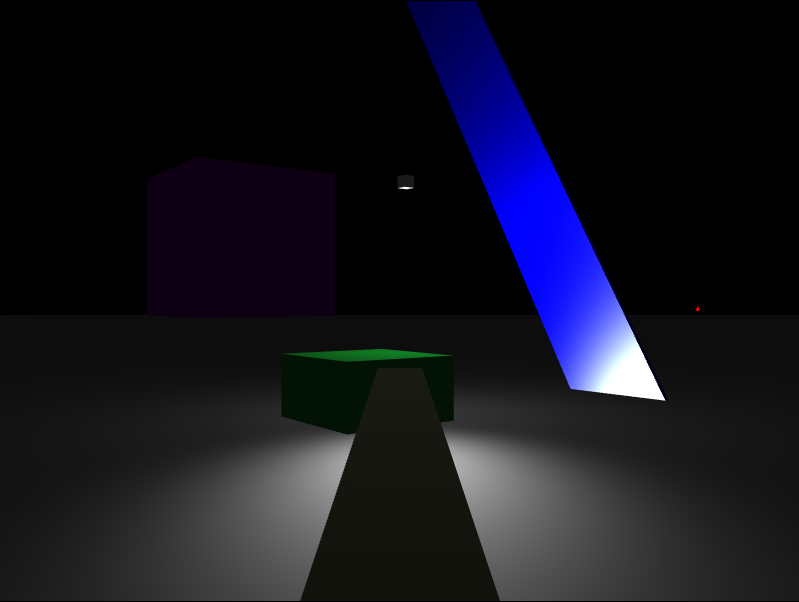
\includegraphics[width=\linewidth]{Cap-Desenvolvimento/gamedoom.png}
  \caption{Jogo implementado utilizando-se a framework}
  \label{des:gamedoom}
\end{figure}

O código desenvolvido pode ser encontrado em \url{https://github.com/Ghust1995/my-cpp-engine/tree/love-like}


\chapter{Documentação}
\label{cap:Documentação}

Nesse capítulo as principais interfaces publicas da aplicação serão explicadas. Como explicado no \nameref{cap:desenvolvimento}, foram implementados duas bibliotecas: \nameref{doc:graphics}, \nameref{doc:time}, e 6 classes: \nameref{doc:game}, \nameref{doc:transform}, \nameref{doc:camera}, \nameref{doc:events}, \nameref{doc:scheduler}, \nameref{doc:keyboardinput}, \nameref{doc:mouseinput},

\section{Classe Game}
\label{doc:game}

A classe game é a classe principal executada pela framework, ela é composta de 3 métodos que devem ser implementados: 

\subsection{void Load()}
Chamada uma única vez no código antes do jogo inicializar qualquer coisa. Essa função tem como intenção alocar as variaveis e coisas que não serão executadas a todo frame.

\subsection{void Update()}
Chamada a todo frame e tem como intenção atualizar as variaveis do jogo.
 
\subsection{void Draw()}
Chamada todo frame com a intenção de desenhar coisas na tela. Essa função é otimizada pra utilizar a biblioteca Graphics.

\section{Classe Transform}
\label{doc:transform}

A classe transform é um container de translação, rotação e escala, tendo também algumas funções auxilares muito usadas com essa informação.

\subsection{Transform()}
O construtor da Classe transform pode receber um vetor de translação, um quaternião de rotação e um vetor de escala.

\subsection{glm::vec3 forward()}
Esse método retorna o vetor (0, 0, -1) rotacionado da rotação da Transform.

\subsection{glm::vec3 up()}
Esse método retorna o vetor (0, 1, 0) rotacionado da rotação da Transform.

\subsection{glm::vec3 right()}
Esse método retorna o vetor (1, 0, 0) rotacionado da rotação da Transform.

\subsection{void Translate(glm::vec3 translation)}
Esse método muda a posição da Transform, fazendo uma translação definida pelo parametro \textit{translation}.

\subsection{void Rotate(float angle, glm::vec3 axis)}
Esse rotaciona a Transform, fazendo uma rotação definida pelo eixo \textit{axis} e pelo angulo \textit{angle}.

\subsection{glm::vec3 position}
A posição da Transform
\subsection{glm::vec3 rotation}
A rotação da Transform
\subsection{glm::vec3 scale}
A escala da Transform

\section{Classe Camera}
\label{doc:camera}

A camera é um objeto utilizado pela biblioteca Graphics para determinar como a cena será renderizada, toda cena deverá possuir pelo menos uma camera.

\subsection{Camera(const float fov, const float aspect\_ratio, const float near, const float far)}
O construtor da camera recebe basicamente as informaçoes sobre o \textit{frustrum}. Cria uma camera na posição (0, 0, 0) e sem rotação (olhando para o eixo z negativo).

\subsection{void Translate(glm::vec3 translation)}
Esse método muda a posição da Transform da camera, fazendo uma translação definida pelo parametro \textit{translation}.
  
\subsection{void Rotate(float angle, glm::vec3 axis)}
Esse rotaciona a Transform da camera, fazendo uma rotação definida pelo eixo \textit{axis} e pelo angulo \textit{angle}.

\subsection{void SetPosition(glm::vec3 position)}
Esse método seta a posição da Transform da camera.

\subsection{void SetRotation(glm::quat rotation)}
Esse método seta a rotação da Transform da camera.

\subsection{glm::vec3 position()}
Esse método pega a posição da Transform da camera.

\subsection{glm::quat rotation()}
Esse método pega a rotação da Transform da camera.

\section{Classe EventSystem}
\label{doc:events}

\subsection{EventSystem()}
Cria um novo event system.

\subsection{void Add(Event e, Callback callback)}
Adiciona um novo callback para quando o evento e for disparado.

\subsection{void Fire(Event e)}
Dispara o evento e.

\section{Classe KeyboardInput}
\label{doc:keyboardinput}
Essa classe serve para transformar inputs do teclado do usuário em funções do jogo.

\subsection{KeyboardInput(SDL\_KeyMapping *keymapping, const int mappingsize)}
O construtor recebe uma lista de mapeamento de teclas para um nome de ação e o tamanho dessa lista.

\subsection{void BindAction(const char *name, const InputType type, const std::function<void()> callback)}
Essa função registra a função callback para ser chamada quando a ação \textit{name}  do tipo \textit{type} for chamada.

InputType pode ser INPUT\_DOWN (quando a tecla é pressionada), INPUT\_UP (quando a tecla é solta)  e INPUT\_HOLD (quando ela está sendo segurada);

\section{Classe MouseInput}
\label{doc:mouseinput}
Essa classe serve para transformar inputs do mouse do usuário em funções do jogo.

\subsection{MouseInput(SDL\_MouseKeyMapping *keymapping, const int mappingsize)}
O construtor recebe uma lista de mapeamento de botões do mouse para um nome de ação e o tamanho dessa lista.

\subsection{void BindAction(const char *name, const InputType type, const std::function<void()> callback)}
Análoga à função BindAction da KeyboardInput.

\subsection{void BindMovement(const std::function<void(const MouseMovementData *d)> callback)}
Registra uma função que recebe informações sobre a movimentação do mouse para ser chamada toda vez que o mouse se movimentar.

\section{Classe Scheduler}
\label{doc:scheduler}
Essa classe serve para fazer chamadas de funções após um tempo em segundos.

\subsection{Scheduler()}
Cria um novo scheduler.

\subsection{void Update(SchedulerTime delta\_time)}
Atualiza o scheduler do tempo que passou. Geralmente o uso disso é chamar ela no Update do Game com delta\_time = Time::GetDelta().

\subsection{void Add(SchedulerTime dt, SchedulerTask task)}
Adiciona a função task para ser chamada após dt segundos.

\subsection{void Repeat(SchedulerTime delay, SchedulerTime dt, SchedulerTask task)}
Adiciona a função task para ser repetida a cada dt segundos, depois de um delay.

\subsection{void Repeat(SchedulerTime dt, SchedulerTask task)}
Adiciona a função task para ser repetida a cada dt segundos (com delay inicial de dt segundos).


\section{Namespace Time}
\label{doc:time}
Namespace com funções globais relacionadas a tempo.

\subsection{float GetDelta()}
Retorna o tempo que passou entre o ultimo frame e o frame atual.

\subsection{float GetTotal()}
Retorna o tempo total de jogo desde sua inicialização.

\section{Namespace Graphics}
\label{doc:graphics}

\subsection{void Cube()}
Existem duas versoes, a Cube(glm::vec3 position, glm::quat rotation = glm::quat(), glm::vec3 scale = glm::vec3(1.0f)), e a Cube(Transform transform), a primeira recebe uma posição, uma rotação e uma escala, e posiciona um cubo, a outra recebe uma Transform e posiciona um cubo baseado nas mesmas informações. Essa função é uma prova de conceito da futura função que importaria um objeto genérico, que nao foi implementada por motivos de simplicidade.

\subsection{void SetMaterial(glm::vec3 diffuse_color, glm::vec3 specular_color)}
Essa função seta o materia que vai ser usado a partir desse momento, dependendo do shader atual, o material pode ou não afetar em propriedades como como a luz interage com o objeto.

\subsection{void PointLight(glm::vec3 position, glm::vec3 color, float intensity)}
Cria uma luz pontual na posicao definida, com cor e intensidade dada pelos parametros. Envia essas informações que podem ou não ser utilizadas pelo atual shader.

\subsection{void SetAmbientLight(glm::vec3 color)}
Seta a luz ambiente para uma determinada cor. Envia essas informações que podem ou não ser utilizadas pelo atual shader.

\subsection{void SetClearColor(glm::vec3 color)}
Seta a cor que é o plano de fundo do jogo (padrão preto).

\subsection{void SetCamera(const Camera *camera)}
Faz com que a atual camera que está renderizando a cena seja a setada por essa função.

\subsection{void Clear()}
Limpa todos os poligonos criados até então.


\chapter{Considerações Finais}

O objetivo geral proposto foi cumprido com sucesso. Foi feita uma implementação de uma framework simples, nos moldes da framework Love2D e XNA, com simplificações. Alem disso foram implementadas algumas funcionalidades não propostas no objetivo que facilitam profundamente a implementação de um jogo, em especial o sistema de eventos e o de chamadas temporais.

O projeto pode ser continuado através da implementação de mais funcionalidades nele para expandir ainda mais o leque de possibilidades de implementação de jogos com a framework.

Algumas funcionalidades já planejadas para a framework são:

\subsection{Alta prioridade}
\begin{itemize}
  \item Permitir o uso de uma biblioteca de UI imediata para permitir alterações em parametros do jogo em tempo real e criação de uma interface de desenvolvimento durante o jogo.
  \item Implementação de um importador de modelos 3d e criação de mais algumas formas geométricas como: triangulo, quadrado, esfera e piramide.
  \item Implementar a utilização de texturas, para que seja possível que os objetos tenham não só uma unica cor, mas desenhos mais complexos.
\end{itemize}

\subsection{Media prioridade}
\begin{itemize}
  \item Fazer com que a camera possa renderizar para lugares diferentes da tela (fazer 2 camera que mostram coisas diferentes em cada metade da tela),
  \item Melhorar a performance para suportar ainda mais objetos em cena.
\end{itemize}

\subsection{Baixa prioridade}
\begin{itemize}
  \item Extensão da interface input\_handler para receber inputs de joysticks, e tambem criação de uma classe KeyboardMouseInput, que junta teclado e mouse em uma única funcionalidade.
  \item Expandindo as melhorias da camera e da textura, porém outra tarefa de igual dificuldade, seria poder colocar a imagem da camera em uma textura, abrindo margem para diversas possibilidades graficas, como espelhos.
\end{itemize}

% REFERENCIAS BIBLIOGRAFICAS
\renewcommand\bibname{\itareferencesnamebabel} %renomear título do capítulo referências
\bibliography{Referencias/referencias}

% Apendices
\appendix
\chapter{Representação Matricial de Pontos, Vetores e Transformações} %opcional
\label{ape:matrix}
\section{Pontos e Vetores}
Model Matrix

Quando se tratando de pontos no espaço tridimensional que serão transformados de diversas formas, é comum utilizar a notação matricial para pontos e vetores de forma que toda transformação se resume a uma multiplicação de matrizes.

Assim, um ponto $p = (p_x, p_y, p_z)$, é representado por:

\begin{equation}
\begin{bmatrix}
    p_x \\
    p_y \\
    p_z \\
    1 \\
\end{bmatrix}
\end{equation}

Analogamente um vetor $v = (v_x, v_y, v_z)$, é representado por:
\begin{equation}
\begin{bmatrix}
    v_x \\
    v_y \\
    v_z \\
    0 \\
\end{bmatrix}
\end{equation}

O quarto elemento da matriz têm algumas propriedades interessantes, que serão demonstradas adiante, mas um primeiro fato relevante é que a subtração de dois pontos resulta num vetor.

Com essa representação matricial de pontos e vetores surgem tambem representações matriciais para diversos tipos de transformações:


\section{Transformações}
\subsection{Translação}

A matriz que define uma translação de $t_x$ no eixo x, $t_y$ no eixo y e $t_z$ no eixo z é definida da seguinte forma:
\begin{equation}
T = 
\begin{bmatrix}
    1 & 0 & 0 & t_x\\
    0 & 1 & 0 & t_y\\
    0 & 0 & 1 & t_z\\
    0 & 0 & 0 & 1 \\
\end{bmatrix}
\end{equation}

Assim, para aplicar uma transformaçao em um ponto basta multiplicar a matriz pelo ponto:
\begin{equation}
\begin{bmatrix}
    1 & 0 & 0 & t_x\\
    0 & 1 & 0 & t_y\\
    0 & 0 & 1 & t_z\\
    0 & 0 & 0 & 1 \\
\end{bmatrix}
*
\begin{bmatrix}
    p_x \\
    p_y \\
    p_z \\
    1 \\
\end{bmatrix}
=
\begin{bmatrix}
    p_x + t_x\\
    p_y + t_y\\
    p_z + t_z\\
    1 \\
\end{bmatrix}
\end{equation}


Da mesma forma, pode-se aplicar uma matriz de translação a um vetor, tendo o seguinte resultado:
\begin{equation}
\begin{bmatrix}
    1 & 0 & 0 & t_x\\
    0 & 1 & 0 & t_y\\
    0 & 0 & 1 & t_z\\
    0 & 0 & 0 & 1 \\
\end{bmatrix}
*
\begin{bmatrix}
    v_x \\
    v_y \\
    v_z \\
    0 \\
\end{bmatrix}
=
\begin{bmatrix}
    v_x\\
    v_y\\
    v_z\\
    0 \\
\end{bmatrix}
\end{equation}

Percebe-se que pela característica de seu ultimo elemento ser 0, a translação não afeta o vetor, sendo esse o comportamento esperado.

\subsection{Escala}

Outra transformação muito comum é a de escalar vetores e pontos. Escala é uma multiplicação termo a termo dos elementos de uma tripla ordenada por outra. A matrix de escala é definida da seguinte forma:

\begin{equation}
S = 
\begin{bmatrix}
    s_x & 0   & 0   & 0\\
    0   & s_y & 0   & 0\\
    0   & 0   & s_z & 0\\
    0   & 0   & 0   & 1 \\
\end{bmatrix}
\end{equation}

No contexto de pontos, a escala afasta o ponto da origem por um fator $s_x$ no eixo x, $s_y$ no eixo y e $s_z$ no eixo z. A aplicação da matrix no ponto é dada pela equação a seguir:
\begin{equation}
\begin{bmatrix}
    s_x & 0   & 0   & 0\\
    0   & s_y & 0   & 0\\
    0   & 0   & s_z & 0\\
    0   & 0   & 0   & 1 \\
\end{bmatrix}
*
\begin{bmatrix}
    p_x\\
    p_y\\
    p_z\\
    1 \\
\end{bmatrix}
=
\begin{bmatrix}
    p_x * s_x\\
    p_y * s_y\\
    p_z * s_z\\
    1 \\
\end{bmatrix}
\end{equation}


De forma análoga, a matriz de escala muda o tamanho do vetor em cada um de seus eixos, sendo sua aplicação dada pelo valor a seguir.
\begin{equation}
\begin{bmatrix}
    s_x & 0   & 0   & 0\\
    0   & s_y & 0   & 0\\
    0   & 0   & s_z & 0\\
    0   & 0   & 0   & 1 \\
\end{bmatrix}
*
\begin{bmatrix}
    v_x\\
    v_y\\
    v_z\\
    0 \\
\end{bmatrix}
=
\begin{bmatrix}
    v_x * s_x\\
    v_y * s_y\\
    v_z * s_z\\
    0 \\
\end{bmatrix}
\end{equation}


\subsection{Rotação}

Rotações são operações complexas, e portanto uma outra matemática foi desenvolvida para ela, a dos quaterniões, que não será explicada em detalhes no presente relatório. No entanto mesmo que o uso de quaterniões para composição e interpolações seja mais simples, os mesmos são transformados em matrizes de rotação e utilizados da mesma forma que as transformações anteriores. Um exemplo da matriz de rotação mais utilizada que é a rotação de um ângulo $\theta$ por um eixo $u = (u_x, u_y, u_z)$, representada a seguir:

\begin{equation}
R = 
\begin{bmatrix}
    \cos\theta + u_x^2(1-\cos\theta) & u_x u_y (1-\cos\theta) - u_z \sin\theta & u_x u_z (1-\cos\theta) - u_y \sin\theta & 0 \\
     u_y u_x (1-\cos\theta) - u_z \sin\theta   & \cos\theta + u_y^2(1-\cos\theta) & u_y u_z (1-\cos\theta) - u_x \sin\theta    & 0\\
     u_z u_x (1-\cos\theta) - u_y \sin\theta &  u_z u_y (1-\cos\theta) - u_x \sin\theta & \cos\theta + u_z^2(1-\cos\theta)  & 0\\
    0   & 0   & 0   & 1 \\
\end{bmatrix}
\end{equation}

\subsection{Projeção}

Outra transformação muito útil na renderização 3d é a de projeção, sendo a mais utilizada delas a de projeção em perspectiva. A matrix de projeção em perspectiva transforma os pontos de forma que distancias em x e y são afetadas pela posição z. Isso torna-se muito mais claro observando as seguintes imagens:

\begin{figure}[]
  \centering
  \subfloat[Antes]{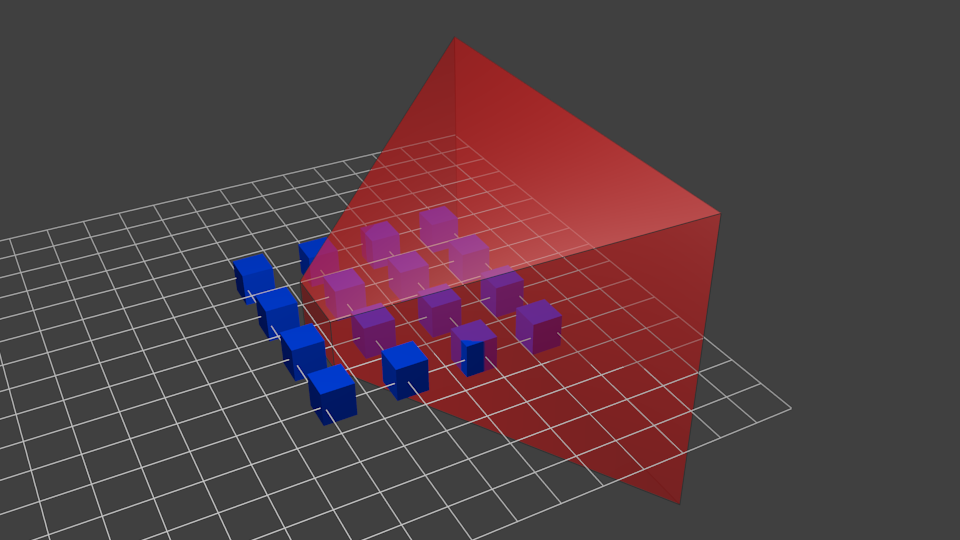
\includegraphics[width=0.45\textwidth]{Ape-Matrizes/perspective-before.png}\label{fig:perspective-before}}
  \hfill
  \subfloat[Depois]{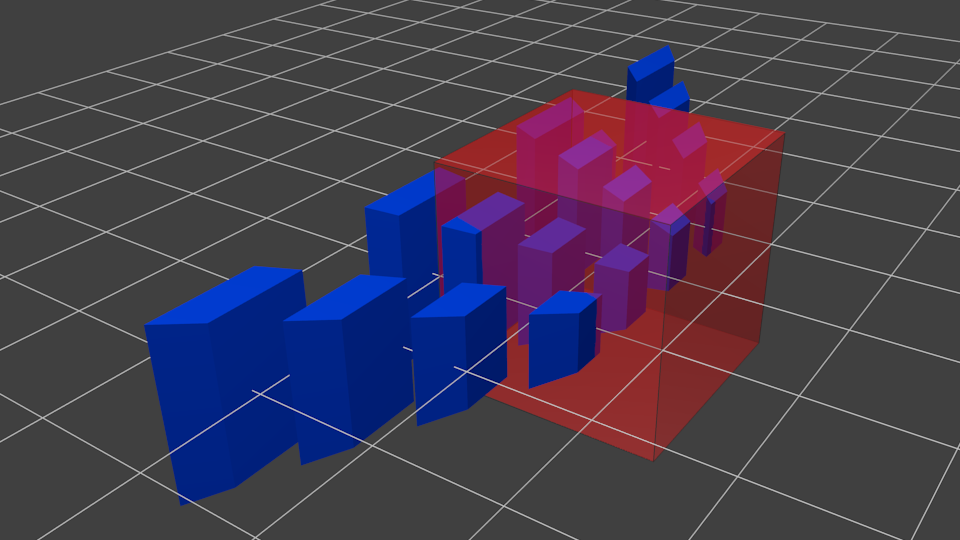
\includegraphics[width=0.45\textwidth]{Ape-Matrizes/perspective-after.png}\label{fig:perspective-after}}
  \caption{Aplicação da matriz de perspectiva a pontos no espaço}
\end{figure}

A matriz de perspectiva geralmente é definida por uma forma conhecida como \textit{frustrum}, um tronco de pirâmide no qual todos os objetos internos são projetados em relação à parte menor. O formato do frustrum pode ser observado na figura \ref{fig:perspective-before}. Para tanto são necessárias alguns parâmetros, a distancia no eixo z do plano proximo (parte menor), representada por $n_z$, a distância no eixo z do plano distante (base), representada por $f_z$, o ângulo de abertura da pirâmide, \textit{fov}, e a razão entre a largura e a altura da base da piramide, representada por \textit{ar}.

Com esses parâmetros, é possível definir a matriz de projeção em perspectiva da seguinte forma:
\begin{equation}
S = 
\begin{bmatrix}
    \frac{1}{ar*\tan(\frac{fov}{2})} & 0 & 0 & 0\\
    0 & \frac{1}{\tan(\frac{fov}{2})} & 0 & 0\\
    0 & 0 & \frac{-n_z-f_z}{n_z-f_z} & 0\\
    0 & 0 & 1 & \frac{2*n_z*f_z}{n_z-f_z}\\
\end{bmatrix}
\end{equation}



% Glossario
%\itaglossary
%\printglossary

% TODO: Folha de Registro do Documento
% Valores dos campos do formulario
\FRDitadata{22 de março de 2017}
\FRDitadocnro{DCTA/ITA/TC-018/2015} %(o número de registro você solicita a biblioteca)
\FRDitaorgaointerno{Instituto Tecnológico de Aeronáutica -- Divisão de Engenharia Mecânica -- ITA/IEM}
%Exemplo no caso de pós-graduação: Instituto Tecnol{\'o}gico de Aeron{\'a}utica -- ITA
\FRDitapalavrasautor{Cupim; Cimento; Estruturas}
\FRDitapalavrasresult{Cupim; Dilema; Construção}
%Exemplo no caso de graduação (TG):
%\FRDitapalavraapresentacao{Trabalho de Graduação, ITA, São José dos Campos, 2015. \NumPenultimaPagina\ páginas.}
%Exemplo no caso de pós-graduação (msc, dsc):
\FRDitapalavraapresentacao{ITA, São José dos Campos. Curso de Mestrado. Programa de Pós-Graduação em Engenharia Aeronáutica e Mecânica. Área de Sistemas Aeroespaciais e Mecatrônica. Orientador: Prof.~Dr. Adalberto Santos Dupont. Coorientadora: Prof$^\textnormal{a}$.~Dr$^\textnormal{a}$. Doralice Serra. Defesa em 05/03/2015. Publicada em 25/03/2015.}
\FRDitaresumo{Aqui começa o resumo do referido trabalho. Não tenho a menor idéia do que colocar aqui. Sendo assim, vou inventar. Lá vai: Este trabalho apresenta uma metodologia de controle de posição das juntas passivas de um manipulador subatuado de uma maneira subótima. O termo subatuado se refere ao fato de que nem todas as juntas ou graus de liberdade do sistema são equipados com atuadores, o que ocorre na prática devido a falhas ou como resultado de projeto. As juntas passivas de manipuladores desse tipo são indiretamente controladas pelo movimento das juntas ativas usando as características de acoplamento da dinâmica de manipuladores. A utilização de redundância de atuação das juntas ativas permite a minimização de alguns critérios, como consumo de energia, por exemplo.
Apesar da estrutura cinemática de manipuladores subatuados ser idêntica a do totalmente atuado, em geral suas caraterísticas dinâmicas diferem devido a presença de juntas passivas. Assim, apresentamos a modelagem dinâmica de um manipulador subatuado e o conceito de índice de acoplamento. Este índice é utilizado na sequência de controle ótimo do \mbox{manipulador}.
A hipótese de que o número de juntas ativas seja maior que o número de
passivas  $(n_{a} > n_{p})$  permite o controle ótimo das juntas passivas, uma vez que na etapa
de controle destas há mais entradas (torques nos atuadores das juntas ativas), que
elementos a controlar (posição das juntas passivas). }
%  Primeiro Parametro: Nacional ou Internacional -- N/I
%  Segundo parametro: Ostensivo, Reservado, Confidencial ou Secreto -- O/R/C/S
\FRDitaOpcoes{N}{O}
% Cria o formulario
\itaFRD

\end{document}
% Fim do Documento. O massacre acabou!!! :-)
